\section{Describing Variation of Time-Dependent Output}\label{sec:sa_time_dependent_variation}

Ramsay and Silverman \cite{Ramsay2005} popularized \gls{fda}, which refers to statistical analyses of data that are functions.
The main assumption of \gls{fda}, as opposed to a more conventional multivariate analysis, is that data present sufficient smoothness, defined by existence of derivatives up to a certain order.
Another distinguishing feature of \gls{fda}, as opposed to time-series analysis or spatial statistics, is the availability of numerous replications of such data (i.e., set of functions) produced by the same or similar underlying process. 
The goal of \gls{fda} related to this work is to describe the overall variation of a set of functions using a smaller set of scalars and functions based on \glsentryfull{pca}.
The functions remain the same for all of the functions in the dataset. 
On the other hand, the scalars vary and, in turn, can be used as the \gls{qoi} for \gls{sa}.

\subsection{Functional Output Representation}\label{sub:sa_spline}

The assumption of continuity within a practically discrete data set (such as the numerical code output of Eq.~(\ref{eq:discrete_time}) is made explicit through a functional representation.
The recommended representation is through a linear combination of basis functions \cite{Ramsay2005}.
This thesis adopts the B-spline basis function \cite{Gillies2010} expansion because of its flexibility \cite{Eilers1996,Eilers2010} 
and the wide availability of its implementation in open numerical libraries \cite{RCT2017}.

Within this framework, a function can be written using basis function expansion as,
\begin{equation}
	y_i (t) = \sum_{k = 1}^{K} c_{ik} \cdot \phi_k (t); \quad i = 1, 2, \cdots N
\label{eq:basis_function_expansion}
\end{equation}
where $K$ indicates the number of basis functions. $\phi_k (t)$ is the $k$-th basis function, 
and $c_{ik}$ is the basis coefficient.
The latter is fitted to the data set to construct curve $i$ with or without smoothing (i.e., interpolating condition vs. penalized ).

A B-spline basis function is a basis system constructed using piecewise polynomial (\emph{spline}) connected at select points in the domain called \emph{knots}.
Let $\boldsymbol{\tau}=\{\tau_k; \, k = 0,1,\cdots, L\}$ be a sequence of knots, non-decreasing numbers that divide the function domain into $L$ sub-intervals.
Within each of these sub-intervals, piecewise polynomial of degree $p$ is defined.
At the interconnection, adjacent polynomials are continuous with derivatives up to $p-1$ matching up.

The basis functions in the B-spline system are determined by the degree of the polynomial $p$ and the knot sequence $\boldsymbol{\tau}=\{\tau_k; \, k = 0,1,\cdots, L\}$.
At the left and right boundaries, several spline basis functions are defined with decreasing continuity up to being discontinuous in both ends.
To satisfy these condition, the endpoints are repeated and augmented into the knot sequence such that
\begin{equation}
	\tau_{-(p-2)} = \cdots = \tau_{0} \leq \tau_{1} \leq \cdots \leq \tau_{L} = \cdots = \tau_{L+(p-2)} 
\label{eq:augmented_knots}
\end{equation}
As such, the augmented knot becomes $\boldsymbol{\tau}=\{\tau_k; k = 0,1,\cdots, L + 2p\}$.
B-spline basis functions of degree $p$ can then be defined recursively on the augmented knot sequence using de Boor - Cox formula as follows, 
\begin{equation}
	\begin{split}
		B^0_k (t) = 
			\begin{cases}
				1, & \tau_k \leq t < \tau_{k+1} \\
			0, & \text{otherwise}
	\end{cases} \\
	B^p_k (t) =  \alpha^p_k (t) B^{p-1}_k + \left[1 - \alpha^p_{k+1} (t)\right] B^{p-1}_{k+1} \\
	\alpha^p_k (t) =
	\begin{cases}
				\frac{t - \tau_k}{\tau_{k+p}-\tau_k}, & \tau_{k+p} \neq \tau_k \\
			  0, & \text{otherwise}
	\end{cases}
	\end{split} 
\label{eq:deboor_cox}
\end{equation}
where $B_k^p (t)$ denotes the $k$-th B-spline of degree $p$.
The degree, $p$, and the number of interior knots, $L-1$, (that is excluding the end points) determine the number of spline basis functions according to $K = p + L$.

Fig.~\ref{fig:b_spline} illustrates all the fourteen spline basis functions of degree $3$ over $10$ uniform interior knots defined in $[0,1]$.
The three leftmost and three rightmost basis functions are less smooth compared to the other (twice continuously differentiable) eight basis functions in the center. 
From leftmost to the right (rightmost to the left) the basis functions are discontinuous, continuous, and once continuously differentiable at the left (right) boundaries, respectively.
\begin{figure}[bth]
	\centering
	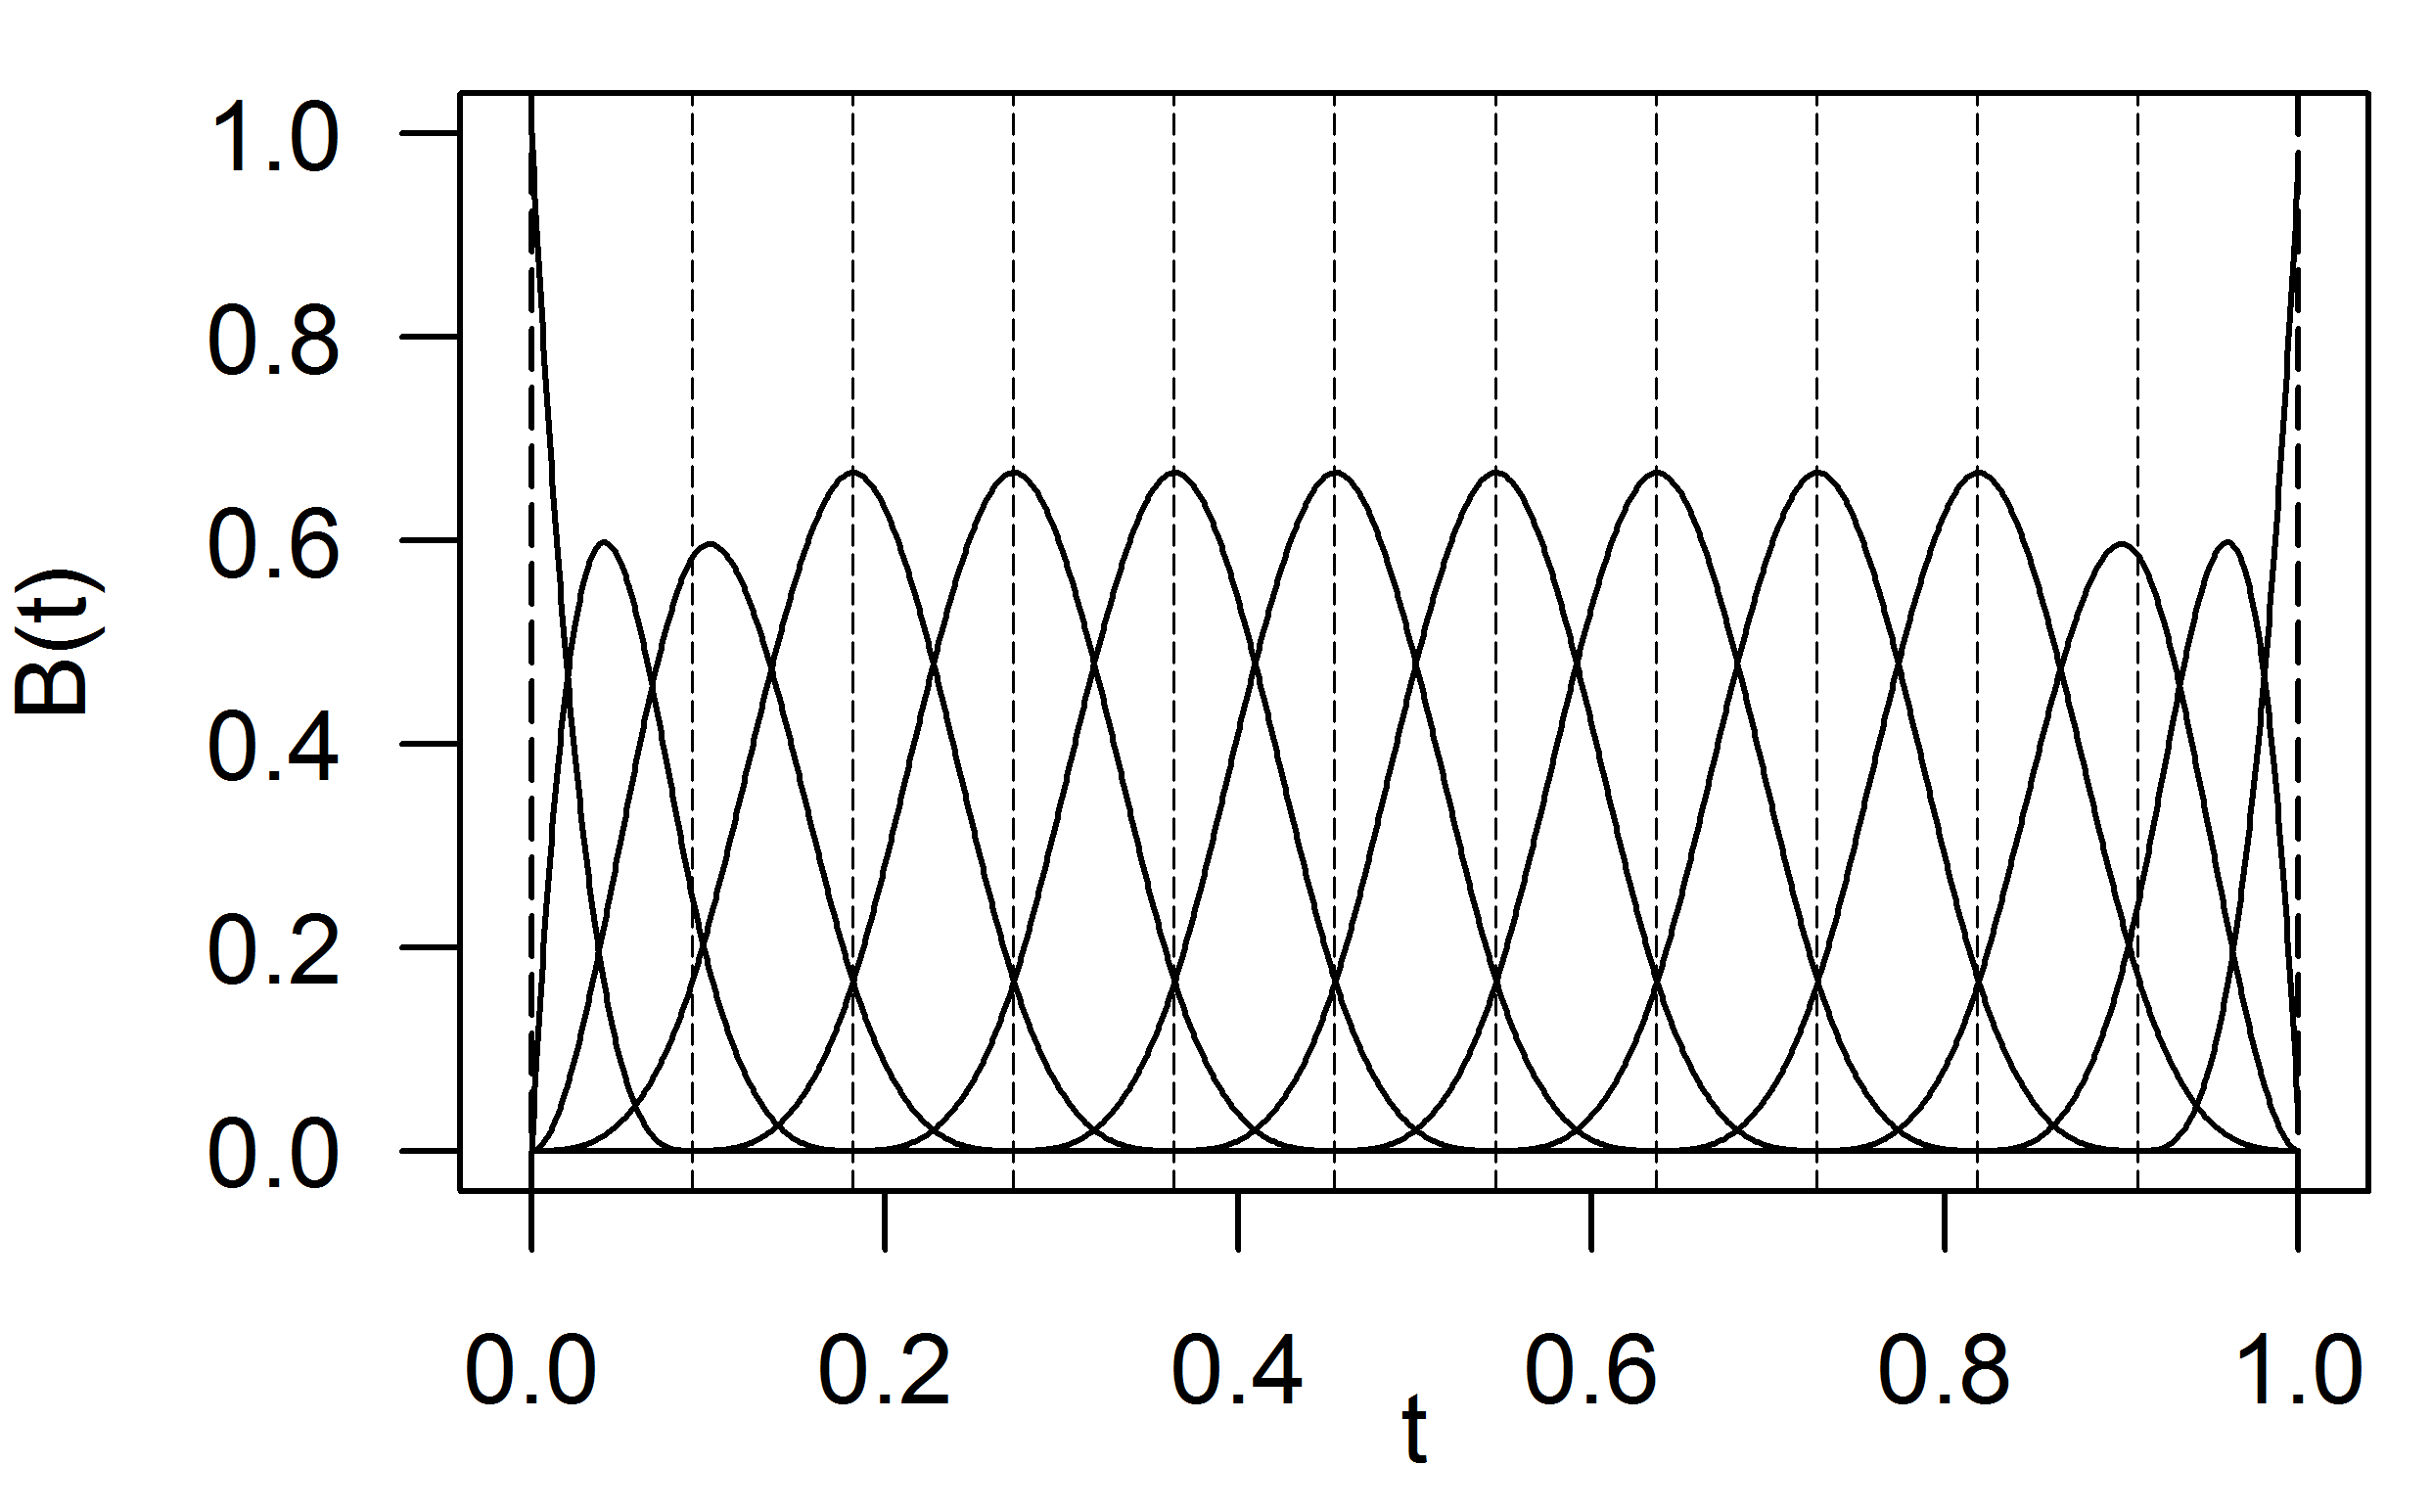
\includegraphics[scale=0.85,trim={0 0.15cm 0 0},clip]{../figures/r-figures/bSpline.png}
	\caption[Spline basis functions of order $4$]{The fourteen spline basis functions of degree $3$ (cubic) with $10$ uniform interior knots (shown in light dashed vertical lines) that divides the domain into 11 sub-intervals}
	\label{fig:b_spline}
\end{figure}

Following Eq.~(\ref{eq:basis_function_expansion}) a function can be written using the B-spline basis functions of a given order $B_k^p (t)$ defined above,
\begin{equation}
	y_i (t) = \sum_{k = 1}^{K} c_{ik} \cdot B^p_k (t); \quad i = 1, 2, \cdots N
\label{eq:basis_function_expansion}
\end{equation}

\subsection{Curve Registration by Landmarks}\label{sub:sa_registration}

Essential to the idea of summary statistics of a data set is the measure of central tendency (e.g., the mean), which characterizes a \emph{typical} realization.
\marginpar{variation in a functional dataset: amplitude \& phase}
The measure of dispersion such as the variance, in turn, is defined relative to the mean. 
Two types of variations are often simultaneously present in a functional data set: 
the variation in magnitude (\emph{vertical} variation) and the variation in phase (\emph{horizontal} variation).
The simultaneous presence of these two types of variations makes even the definition of a mean function difficult \cite{Kneip1992}.

Fig.~\ref{fig:illustrate_phase_variation} illustrates this point.
For a functional data set that does not contain strong phase variations, 
a simple cross-sectional mean (average values across realizations taken at every argument values) does indeed represents a typical realization (Fig.~\ref{fig:illustrate_phase_variation}~left).
On the other hand, with a strong phase variation (often mixed with amplitude variation), 
the cross-sectional mean failed to produce a typical realization (Fig.~\ref{fig:illustrate_phase_variation}~right).
In this case, according to Kneip (\cite{Kneip1992}) a more proper \emph{structural} mean of the data set can be defined instead by first separating the phase and amplitude variations.
\begin{figure}[bth]
	\centering
	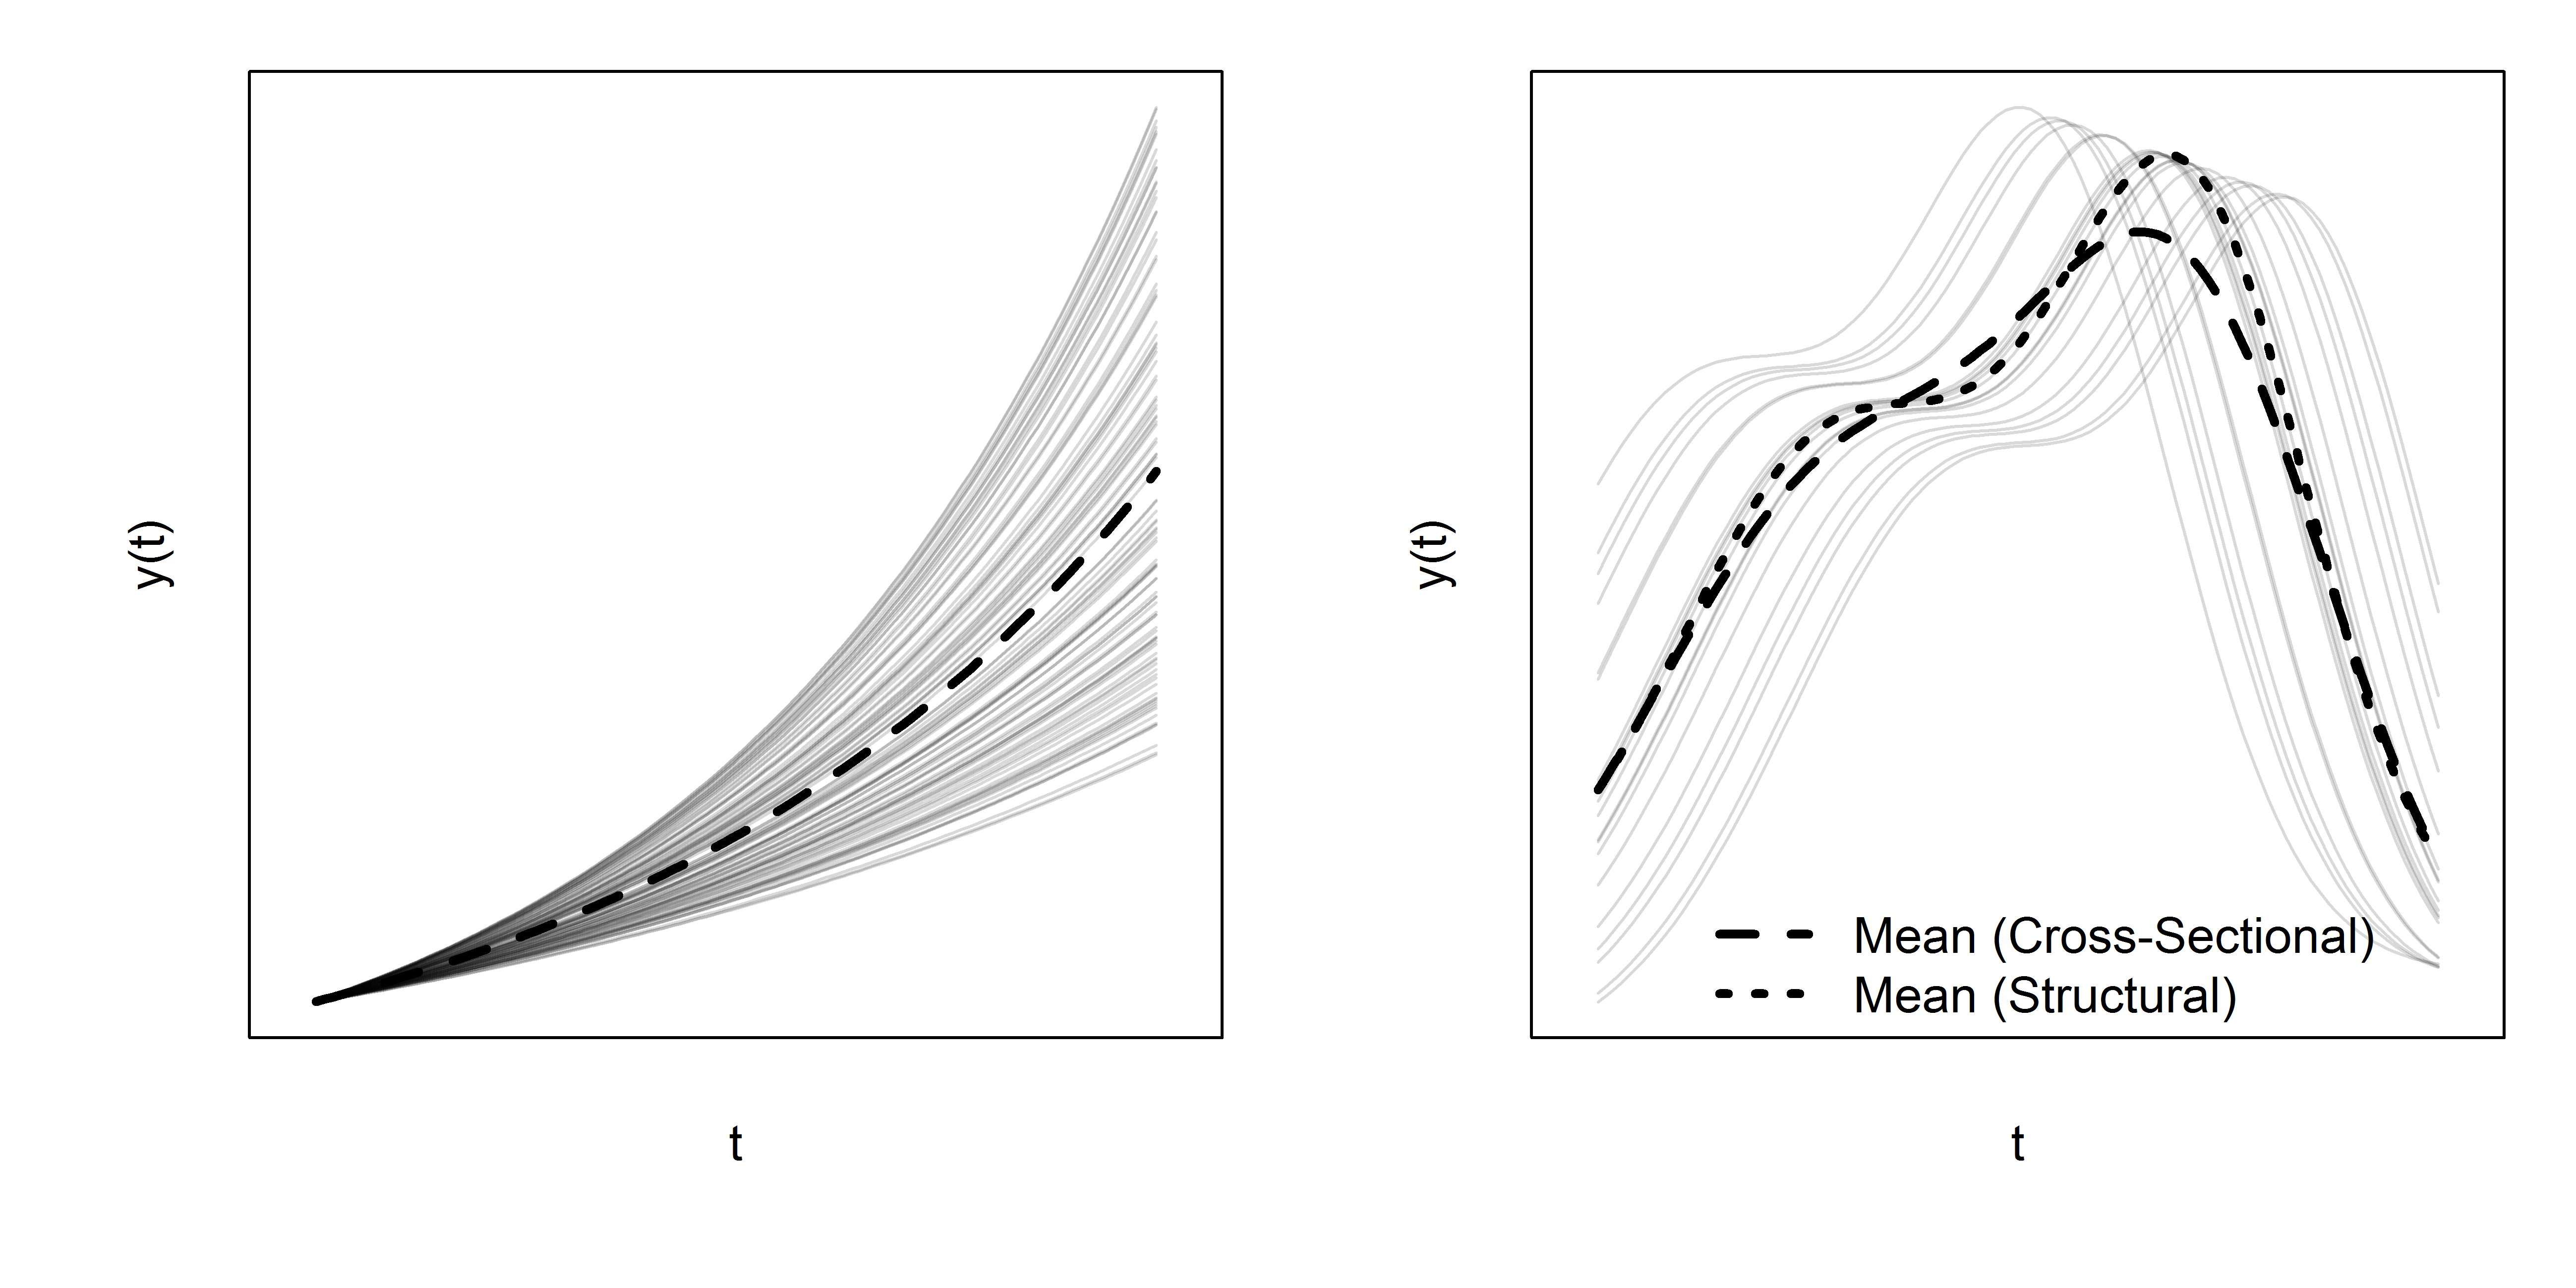
\includegraphics[scale=0.48,trim={0 1cm 0 0},clip]{../figures/r-figures/illustratePhaseVariation.png}
	\caption[Variation in functional data sets, with and without phase variation]{Two examples of functional data sets. (Left) without pronounced phase variation, cross-sectional mean can reflect a typical realization. (Right) with pronounced phase variations, cross-sectional mean differs from the notion of typical realization. \emph{Structural} mean derived after registration better represents a typical realization. The scales in the axes are arbitrary.}
	\label{fig:illustrate_phase_variation}
\end{figure}

In the presence of strong amplitude and phase variation, to obtain the structural mean the two types of variation are first separated through a \emph{registration} procedure \cite{Wang1997,Ramsay1998}.
\marginpar{landmark registration}
The procedure transforms the time argument using a warping function to reduce the phase variation in the dataset.
Specifically, the landmark type registration type is employed because the main features of the function of interest (i.e., reflood curve) are readily identifiable.
In a functional data set with phase variation, this particular type of registration forces important events in a curve (its \emph{landmarks}) to occur at the same time relative to a set of reference values.

This is illustrated in Fig.~\ref{fig:illustrate_registered_curves}.
The left panel shows the functional data set with its phase variation to be reduced by aligning its landmark (i.e., the time of maximum) to a reference value 
(shown as the vertical lines, solid and dashed for the landmarks of realizations and reference, respectively).
The structural mean was computed from the cross-sectional mean of registered curves shown in both panels as dashed curve. 
Indeed, this mean is more representative as a typical realization of the curves in the original dataset.
\begin{figure}[bth!]
	\centering
	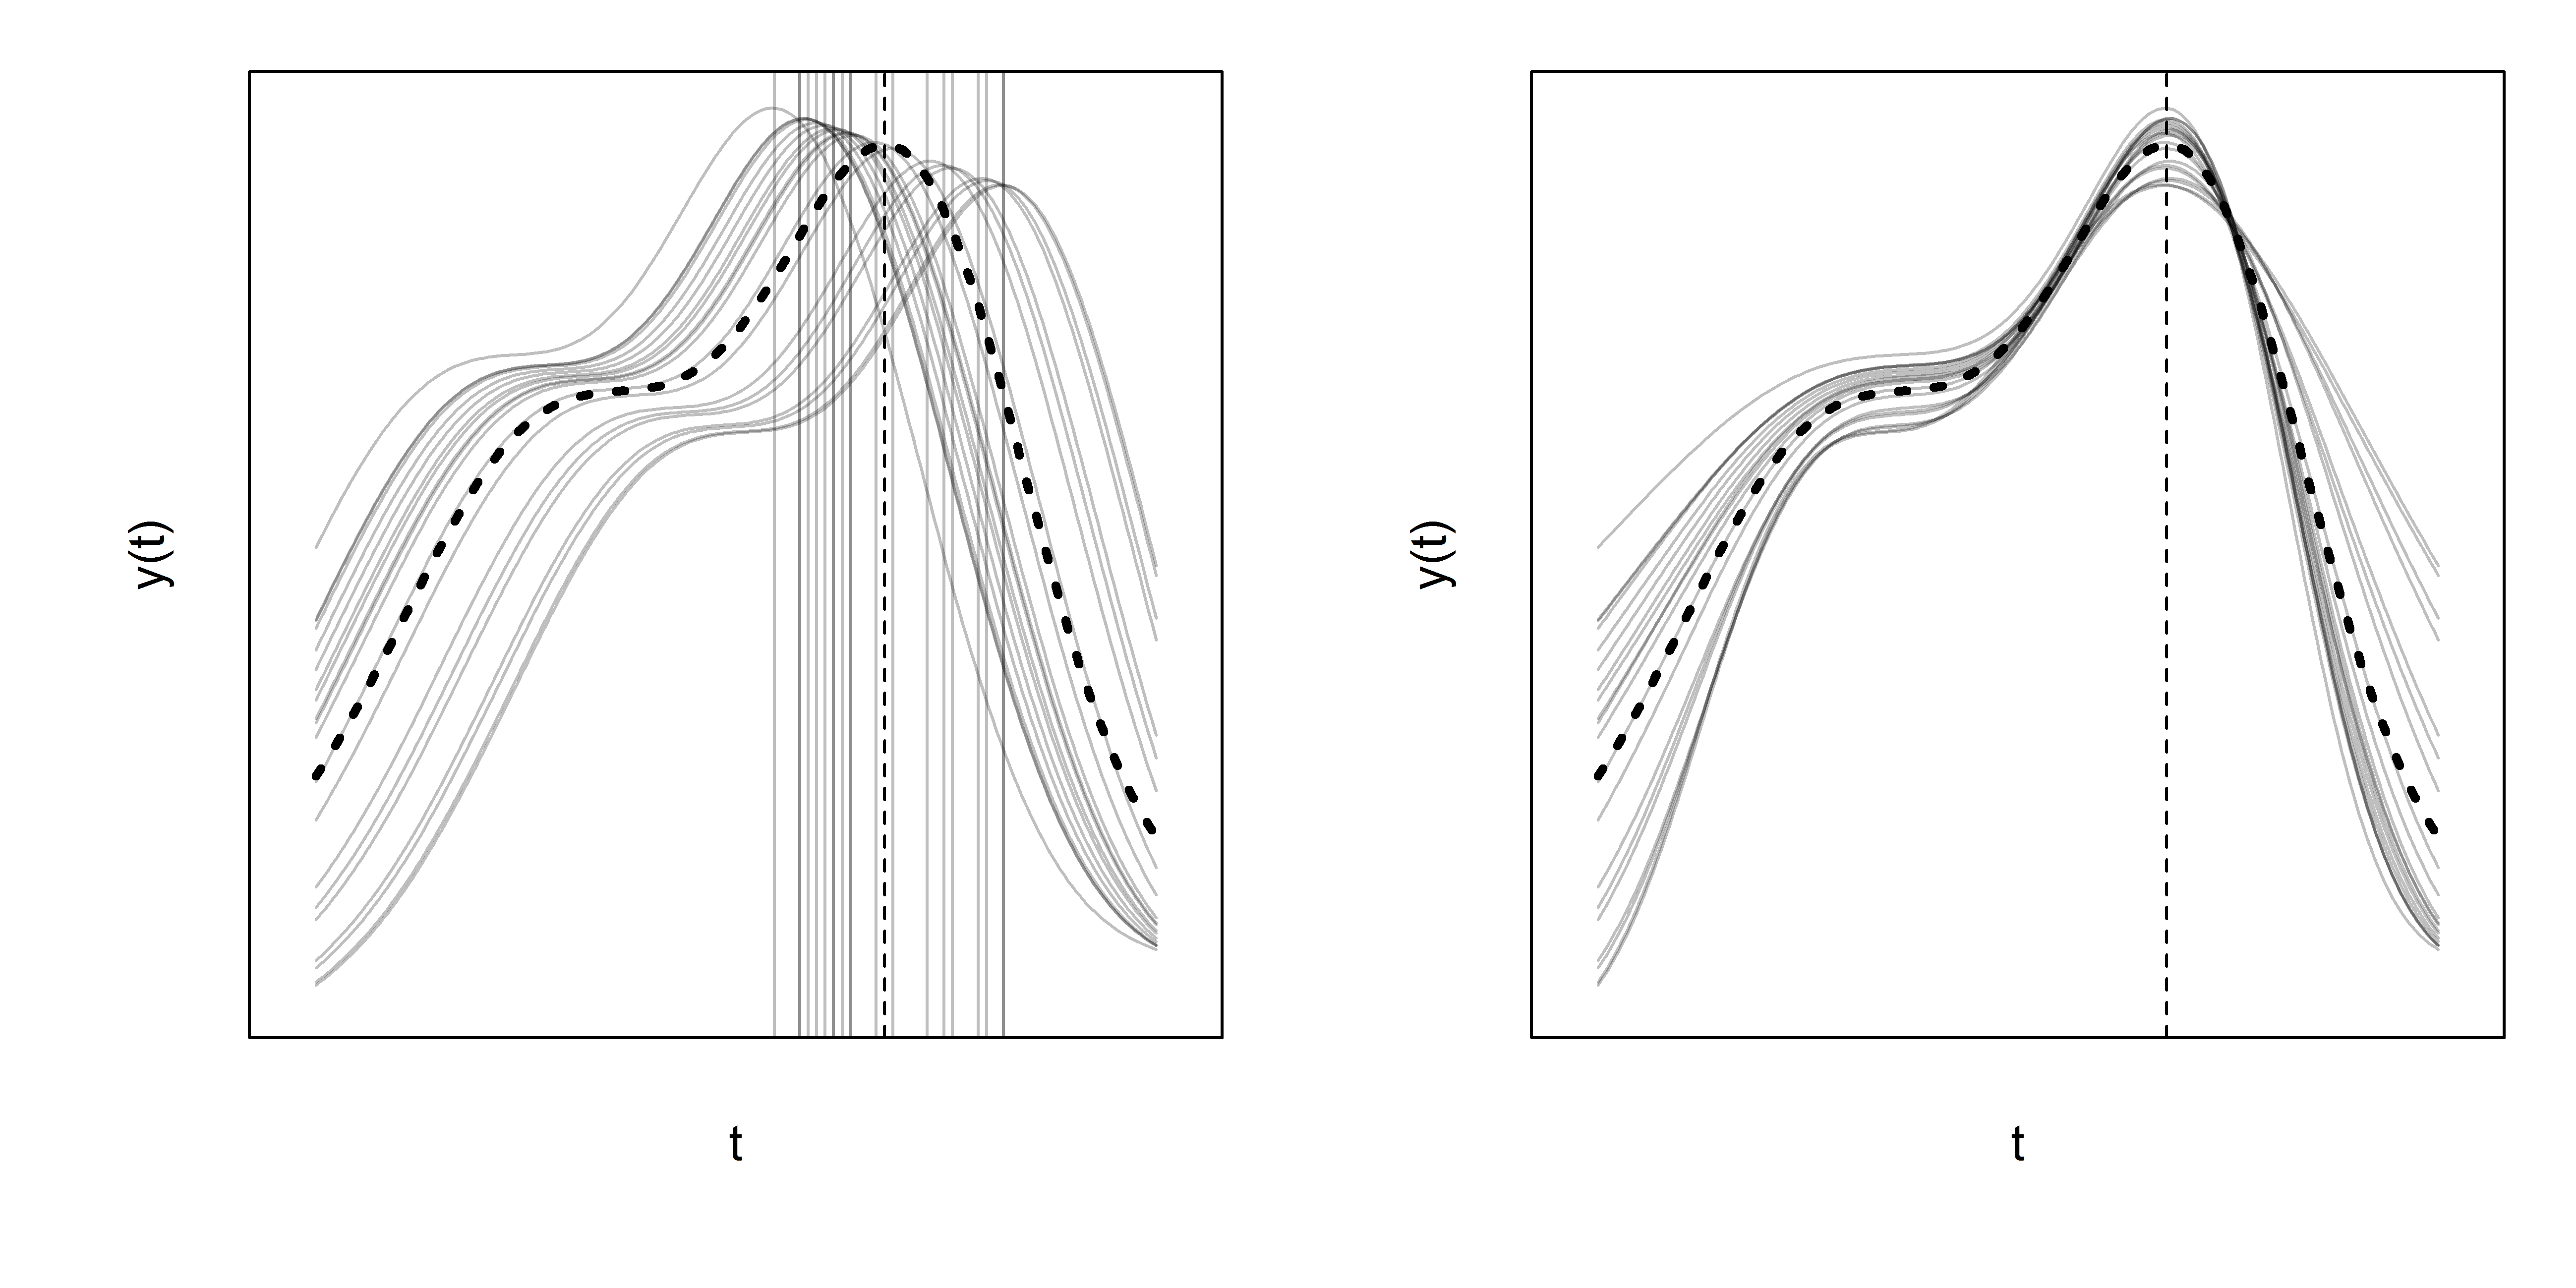
\includegraphics[scale=0.48,trim={0 1cm 0 0},clip]{../figures/r-figures/illustrateRegisteredCurves.png}
	\caption[Illustration of curve registration]{Illustration of curve registration. (Left) curves whose landmarks (solid vertical lines) are to be aligned with respect to a reference value (dashed vertical line). (Right) the registered curves where all curves have been aligned to each other. The structural mean is shown as dashed curve. The scales in the axes are arbitrary.}
	\label{fig:illustrate_registered_curves}
\end{figure}

More details on the properties of the warping functions used to transform the time argument for registration can be found in Appendix~\ref{app:landmark}.

\subsection{Functional Principal Component Analysis}\label{sub:sa_fpca}

Separation of phase variation from magnitude variation by registration procedure allows for the definition of a proper mean function.
With respect to the mean, the notion of functional variation can then be defined.
The covariance function of a set of function realizations $\{y_n(t);n = 1, 2, \cdots, N; t \in [t_a,t_b]\}$ from a random process $Y$ is defined as
\begin{equation}
	\nu (t_1, t_2) \equiv \frac{1}{N} \sum_{n=1}^{N} (y_n(t_1) - \bar{y}(t_1)) \cdot (y_n(t_2) - \bar{y}(t_2))
\label{eq:covariance_function}
\end{equation}
where $\bar{y} (t)$ is the proper mean function.

To extract more meaningful information from the covariance function, the function is often projected onto lower-dimensional space using an orthogonal decomposition.
This projection can be done through the functional principal component (fPC) analysis (fPCA) (also know as the Karhunen-Lo\'eve transform):
\begin{equation}
	\nu (t_1, t_2) = \sum_{j=1}^{+\infty} \rho_j \cdot \xi_j(t_1) \cdot \xi_j(t_2)
\label{eq:kl_transform}
\end{equation}
where $\rho_j$ is a series of ordered eigenvalues of decreasing values; 
$\xi_j(t)$ is the corresponding series of orthogonal eigenfunctions (or the fPC).

The transformation of the covariance function into pairs of eigenvalues and eigenfunctions also allows each element of the original dataset $\{y_n(t)\}$ to be represented as a series that is optimal in the root-mean-square-of-error sense:
\begin{equation}
  y_n(t) = \bar{y}(t) + \sum_{j=1}^{+\infty} \theta_{j,n} \cdot \xi_j (t); \quad n = 1, 2, \cdots, N
\label{eq:pod}
\end{equation}
where the fPC score $\theta_{j,n}$ associated with each realized function is defined by the orthogonality condition
\begin{equation}
  \theta_{j,n} = \int_{t_a}^{t_b} \left[y_n(t) - \bar{y}(t)\right] \cdot \xi_j (t) dt
\label{eq:pod_orthogonality}
\end{equation}

Eqs.~(\ref{eq:pod}) and (\ref{eq:pod_orthogonality}) imply that across realizations in the samples, 
$\{y_n(t)\}$ can be represented linearly using a common mean function and sums of deviation terms from the mean.
The deviation terms consist of a set of common eigenfunctions and a set of fPC scores.
As such, the random character of each realization is left to the score associated with each component and each realization.
Put differently, the eigenfunctions described the (common) modes of variations, 
while the scores quantify the strength of a particular mode~\cite{Wang2012}.
These scores will be used as the \gls{qoi} in the subsequent global \gls{sa}.